% Options for packages loaded elsewhere
\PassOptionsToPackage{unicode}{hyperref}
\PassOptionsToPackage{hyphens}{url}
\PassOptionsToPackage{dvipsnames,svgnames,x11names}{xcolor}
%
\documentclass[
  letterpaper,
  DIV=11,
  numbers=noendperiod]{scrartcl}

\usepackage{amsmath,amssymb}
\usepackage{lmodern}
\usepackage{iftex}
\ifPDFTeX
  \usepackage[T1]{fontenc}
  \usepackage[utf8]{inputenc}
  \usepackage{textcomp} % provide euro and other symbols
\else % if luatex or xetex
  \usepackage{unicode-math}
  \defaultfontfeatures{Scale=MatchLowercase}
  \defaultfontfeatures[\rmfamily]{Ligatures=TeX,Scale=1}
\fi
% Use upquote if available, for straight quotes in verbatim environments
\IfFileExists{upquote.sty}{\usepackage{upquote}}{}
\IfFileExists{microtype.sty}{% use microtype if available
  \usepackage[]{microtype}
  \UseMicrotypeSet[protrusion]{basicmath} % disable protrusion for tt fonts
}{}
\makeatletter
\@ifundefined{KOMAClassName}{% if non-KOMA class
  \IfFileExists{parskip.sty}{%
    \usepackage{parskip}
  }{% else
    \setlength{\parindent}{0pt}
    \setlength{\parskip}{6pt plus 2pt minus 1pt}}
}{% if KOMA class
  \KOMAoptions{parskip=half}}
\makeatother
\usepackage{xcolor}
\usepackage[normalem]{ulem}
\setlength{\emergencystretch}{3em} % prevent overfull lines
\setcounter{secnumdepth}{-\maxdimen} % remove section numbering
% Make \paragraph and \subparagraph free-standing
\ifx\paragraph\undefined\else
  \let\oldparagraph\paragraph
  \renewcommand{\paragraph}[1]{\oldparagraph{#1}\mbox{}}
\fi
\ifx\subparagraph\undefined\else
  \let\oldsubparagraph\subparagraph
  \renewcommand{\subparagraph}[1]{\oldsubparagraph{#1}\mbox{}}
\fi

\usepackage{color}
\usepackage{fancyvrb}
\newcommand{\VerbBar}{|}
\newcommand{\VERB}{\Verb[commandchars=\\\{\}]}
\DefineVerbatimEnvironment{Highlighting}{Verbatim}{commandchars=\\\{\}}
% Add ',fontsize=\small' for more characters per line
\usepackage{framed}
\definecolor{shadecolor}{RGB}{241,243,245}
\newenvironment{Shaded}{\begin{snugshade}}{\end{snugshade}}
\newcommand{\AlertTok}[1]{\textcolor[rgb]{0.68,0.00,0.00}{#1}}
\newcommand{\AnnotationTok}[1]{\textcolor[rgb]{0.37,0.37,0.37}{#1}}
\newcommand{\AttributeTok}[1]{\textcolor[rgb]{0.40,0.45,0.13}{#1}}
\newcommand{\BaseNTok}[1]{\textcolor[rgb]{0.68,0.00,0.00}{#1}}
\newcommand{\BuiltInTok}[1]{\textcolor[rgb]{0.00,0.23,0.31}{#1}}
\newcommand{\CharTok}[1]{\textcolor[rgb]{0.13,0.47,0.30}{#1}}
\newcommand{\CommentTok}[1]{\textcolor[rgb]{0.37,0.37,0.37}{#1}}
\newcommand{\CommentVarTok}[1]{\textcolor[rgb]{0.37,0.37,0.37}{\textit{#1}}}
\newcommand{\ConstantTok}[1]{\textcolor[rgb]{0.56,0.35,0.01}{#1}}
\newcommand{\ControlFlowTok}[1]{\textcolor[rgb]{0.00,0.23,0.31}{#1}}
\newcommand{\DataTypeTok}[1]{\textcolor[rgb]{0.68,0.00,0.00}{#1}}
\newcommand{\DecValTok}[1]{\textcolor[rgb]{0.68,0.00,0.00}{#1}}
\newcommand{\DocumentationTok}[1]{\textcolor[rgb]{0.37,0.37,0.37}{\textit{#1}}}
\newcommand{\ErrorTok}[1]{\textcolor[rgb]{0.68,0.00,0.00}{#1}}
\newcommand{\ExtensionTok}[1]{\textcolor[rgb]{0.00,0.23,0.31}{#1}}
\newcommand{\FloatTok}[1]{\textcolor[rgb]{0.68,0.00,0.00}{#1}}
\newcommand{\FunctionTok}[1]{\textcolor[rgb]{0.28,0.35,0.67}{#1}}
\newcommand{\ImportTok}[1]{\textcolor[rgb]{0.00,0.46,0.62}{#1}}
\newcommand{\InformationTok}[1]{\textcolor[rgb]{0.37,0.37,0.37}{#1}}
\newcommand{\KeywordTok}[1]{\textcolor[rgb]{0.00,0.23,0.31}{#1}}
\newcommand{\NormalTok}[1]{\textcolor[rgb]{0.00,0.23,0.31}{#1}}
\newcommand{\OperatorTok}[1]{\textcolor[rgb]{0.37,0.37,0.37}{#1}}
\newcommand{\OtherTok}[1]{\textcolor[rgb]{0.00,0.23,0.31}{#1}}
\newcommand{\PreprocessorTok}[1]{\textcolor[rgb]{0.68,0.00,0.00}{#1}}
\newcommand{\RegionMarkerTok}[1]{\textcolor[rgb]{0.00,0.23,0.31}{#1}}
\newcommand{\SpecialCharTok}[1]{\textcolor[rgb]{0.37,0.37,0.37}{#1}}
\newcommand{\SpecialStringTok}[1]{\textcolor[rgb]{0.13,0.47,0.30}{#1}}
\newcommand{\StringTok}[1]{\textcolor[rgb]{0.13,0.47,0.30}{#1}}
\newcommand{\VariableTok}[1]{\textcolor[rgb]{0.07,0.07,0.07}{#1}}
\newcommand{\VerbatimStringTok}[1]{\textcolor[rgb]{0.13,0.47,0.30}{#1}}
\newcommand{\WarningTok}[1]{\textcolor[rgb]{0.37,0.37,0.37}{\textit{#1}}}

\providecommand{\tightlist}{%
  \setlength{\itemsep}{0pt}\setlength{\parskip}{0pt}}\usepackage{longtable,booktabs,array}
\usepackage{calc} % for calculating minipage widths
% Correct order of tables after \paragraph or \subparagraph
\usepackage{etoolbox}
\makeatletter
\patchcmd\longtable{\par}{\if@noskipsec\mbox{}\fi\par}{}{}
\makeatother
% Allow footnotes in longtable head/foot
\IfFileExists{footnotehyper.sty}{\usepackage{footnotehyper}}{\usepackage{footnote}}
\makesavenoteenv{longtable}
\usepackage{graphicx}
\makeatletter
\def\maxwidth{\ifdim\Gin@nat@width>\linewidth\linewidth\else\Gin@nat@width\fi}
\def\maxheight{\ifdim\Gin@nat@height>\textheight\textheight\else\Gin@nat@height\fi}
\makeatother
% Scale images if necessary, so that they will not overflow the page
% margins by default, and it is still possible to overwrite the defaults
% using explicit options in \includegraphics[width, height, ...]{}
\setkeys{Gin}{width=\maxwidth,height=\maxheight,keepaspectratio}
% Set default figure placement to htbp
\makeatletter
\def\fps@figure{htbp}
\makeatother
\newlength{\cslhangindent}
\setlength{\cslhangindent}{1.5em}
\newlength{\csllabelwidth}
\setlength{\csllabelwidth}{3em}
\newlength{\cslentryspacingunit} % times entry-spacing
\setlength{\cslentryspacingunit}{\parskip}
\newenvironment{CSLReferences}[2] % #1 hanging-ident, #2 entry spacing
 {% don't indent paragraphs
  \setlength{\parindent}{0pt}
  % turn on hanging indent if param 1 is 1
  \ifodd #1
  \let\oldpar\par
  \def\par{\hangindent=\cslhangindent\oldpar}
  \fi
  % set entry spacing
  \setlength{\parskip}{#2\cslentryspacingunit}
 }%
 {}
\usepackage{calc}
\newcommand{\CSLBlock}[1]{#1\hfill\break}
\newcommand{\CSLLeftMargin}[1]{\parbox[t]{\csllabelwidth}{#1}}
\newcommand{\CSLRightInline}[1]{\parbox[t]{\linewidth - \csllabelwidth}{#1}\break}
\newcommand{\CSLIndent}[1]{\hspace{\cslhangindent}#1}

\KOMAoption{captions}{tableheading}
\makeatletter
\makeatother
\makeatletter
\makeatother
\makeatletter
\@ifpackageloaded{caption}{}{\usepackage{caption}}
\AtBeginDocument{%
\ifdefined\contentsname
  \renewcommand*\contentsname{Table of contents}
\else
  \newcommand\contentsname{Table of contents}
\fi
\ifdefined\listfigurename
  \renewcommand*\listfigurename{List of Figures}
\else
  \newcommand\listfigurename{List of Figures}
\fi
\ifdefined\listtablename
  \renewcommand*\listtablename{List of Tables}
\else
  \newcommand\listtablename{List of Tables}
\fi
\ifdefined\figurename
  \renewcommand*\figurename{Figure}
\else
  \newcommand\figurename{Figure}
\fi
\ifdefined\tablename
  \renewcommand*\tablename{Table}
\else
  \newcommand\tablename{Table}
\fi
}
\@ifpackageloaded{float}{}{\usepackage{float}}
\floatstyle{ruled}
\@ifundefined{c@chapter}{\newfloat{codelisting}{h}{lop}}{\newfloat{codelisting}{h}{lop}[chapter]}
\floatname{codelisting}{Listing}
\newcommand*\listoflistings{\listof{codelisting}{List of Listings}}
\makeatother
\makeatletter
\@ifpackageloaded{caption}{}{\usepackage{caption}}
\@ifpackageloaded{subcaption}{}{\usepackage{subcaption}}
\makeatother
\makeatletter
\@ifpackageloaded{tcolorbox}{}{\usepackage[many]{tcolorbox}}
\makeatother
\makeatletter
\@ifundefined{shadecolor}{\definecolor{shadecolor}{rgb}{.97, .97, .97}}
\makeatother
\makeatletter
\makeatother
\ifLuaTeX
  \usepackage{selnolig}  % disable illegal ligatures
\fi
\IfFileExists{bookmark.sty}{\usepackage{bookmark}}{\usepackage{hyperref}}
\IfFileExists{xurl.sty}{\usepackage{xurl}}{} % add URL line breaks if available
\urlstyle{same} % disable monospaced font for URLs
\hypersetup{
  pdftitle={Open-Source machine learning BANTER acoustic classification of a cryptic echolocating species},
  pdfauthor={Shannon Rankin; Taiki Sakai; Frederick Archer; Jay Barlow; Danielle Cholewiak; Annamaria DeAngelis; Jennifer L. K. McCullough; Erin Oleson; Melissa Soldevilla},
  pdfkeywords={bioacoustics, machine learning, random forest, species
classification, marine mammals, passive acoustic monitoring, beaked
whale},
  colorlinks=true,
  linkcolor={blue},
  filecolor={Maroon},
  citecolor={Blue},
  urlcolor={Blue},
  pdfcreator={LaTeX via pandoc}}

\title{Open-Source machine learning BANTER acoustic classification of a
cryptic echolocating species}
\author{Shannon Rankin \and Taiki Sakai \and Frederick Archer \and Jay
Barlow \and Danielle Cholewiak \and Annamaria DeAngelis \and Jennifer L.
K. McCullough \and Erin Oleson \and Melissa Soldevilla}
\date{2/6/23}

\begin{document}
\maketitle
\begin{abstract}
Passive acoustic monitoring is increasingly used for assessing
populations of marine mammals; however, analysis of large datasets is
limited by our ability to easily classify sounds detected.
Classification of beaked whale acoustic events, in particular, require
evaluation of multiple lines of evidence by expert analysts. Here we
present a highly automated approach to acoustic detection and
classification using supervised machine learning and open source
software methods. Data from four large scale surveys of beaked whales
(North Atlantic, South Atlantic, Hawaii, and Eastern Pacific) were
analyzed PAMGuard (acoustic detection), PAMpal (acoustic analysis) and
BANTER (hierarchical random forest classifier). Overall correct
classification results ranged from 86\% for the South Atlantic data to
99\% for the North Atlantic. Results for many species could likely be
improved with increased sample sizes and consideration of alternative
automated detectors. These methods provide a highly automated approach
to acoustic detection and classification using open source methods that
can be readily adopted for species and geographic regions.
\end{abstract}
\ifdefined\Shaded\renewenvironment{Shaded}{\begin{tcolorbox}[breakable, frame hidden, sharp corners, interior hidden, enhanced, borderline west={3pt}{0pt}{shadecolor}, boxrule=0pt]}{\end{tcolorbox}}\fi

\begin{Shaded}
\begin{Highlighting}[]
\FunctionTok{library}\NormalTok{(tidyverse)}
\end{Highlighting}
\end{Shaded}

\begin{verbatim}
-- Attaching packages --------------------------------------- tidyverse 1.3.2 --
v ggplot2 3.4.0      v purrr   1.0.1 
v tibble  3.1.8      v dplyr   1.0.10
v tidyr   1.2.1      v stringr 1.5.0 
v readr   2.1.3      v forcats 1.0.0 
-- Conflicts ------------------------------------------ tidyverse_conflicts() --
x dplyr::filter() masks stats::filter()
x dplyr::lag()    masks stats::lag()
\end{verbatim}

\begin{Shaded}
\begin{Highlighting}[]
\FunctionTok{library}\NormalTok{(knitr)}
\FunctionTok{library}\NormalTok{(here)}
\end{Highlighting}
\end{Shaded}

\begin{verbatim}
here() starts at C:/Users/shannon.rankin/Documents/GitHub/BANTER_BeakedWhales
\end{verbatim}

\hypertarget{introduction}{%
\section{Introduction}\label{introduction}}

Passive acoustic monitoring (PAM) from has proven to be a valuable tool
for studying populations of marine mammals ((Parijs et al. 2009));
however, the value of these studies depends on our ability to identify
the sources of the sounds we are monitoring. Historically, experienced
acousticians manually identify stereotyped sounds that could be reliably
attributed to a given species, based on their spectral or temporal
characteristics ((Baumann-Pickering et al. 2013a); (Bittle and Duncan
2013); (Rankin and Barlow 2005); (Soldevilla et al. 2008)). The dramatic
increase in recordings make it impossible for experienced acousticians
to manually annotate all data, and there has been an increasing need for
the development of automated classification routines that can provide
accurate determinations of the species responsible for the sounds.

Beaked whales are deep diving marine mammals found in offshore waters;
their long dive intervals and cryptic surfacing behavior make them
difficult to study using typical shipboard visual observation methods
((MacLeod 2018)). However, beaked whales make stereotyped echolocation
clicks that have temporal and spatial characteristics that can be used
to differentiate species ((Baumann-Pickering et al. 2013b)). Detection
of beaked whale signals in large datasets is greatly expanding our
understanding of their population structure and the potential impact of
human activities on these species ((Barlow et al. 2022);
(Baumann-Pickering et al. 2014); (Simonis et al. 2020)). Unfortunately,
manual classification of beaked whale echolocation clicks requires
analysis by trained observers using a number of visual aids to examine
the call characteristics. Development of automated classification
routines, if accurate, serve to improve the efficiency and decrease the
cost of analyzing large datasets.

BANTER is a supervised machine learning acoustic event classifier
originally developed for classifying dolphin schools from acoustic
recordings ((Rankin et al. 2017a)). This hierarchical random forest
event classifier relies on an initial call classifier (in the dolphin
case study, this included one each for whistles, echolocation clicks,
and burst pulses) followed by an event classifier. The event classifier
considers the probability of assignment to species for each call in the
call classifier, along with any event-level characteristics (such as
call rate). BANTER is very flexible and can accommodate any number of
measures from any number of detectors. While BANTER relies on multiple
call types, relatively minor changes to a call detector could yield
different detector results ((Rankin et al. 2017b)). In this case,
settings for a whistle \& moan detector were modified to improve
performance at detecting burst pulses. This approach of applying
multiple call detectors (of the same type but with different settings)
suggests that perhaps BANTER could be used on species that only produce
one call type (or where only one call type was analyzed), as long as the
settings of the automated call detector were modified such that the
overall number of detections was different. This approach was
successfully applied to classified echolocation clicks for narwhal and
belugas ((Zahn et al. 2021)). For species who primarily (or exclusively)
produce echolocation clicks, BANTER may serve as an option for automated
machine learning classification.

Here we applied BANTER acoustic classification to beaked whale
detections from four large acoustic datasets off the US East Coast,
Hawaii, and the US West Coast. Acoustic data were analyzed by
experienced acousticians to determine species identity, and these
`ground truth' classifications served as training data for the
supervised BANTER trials. Our goals are to identify an efficient and
accurate automated approach to acoustic classification of beaked whales,
and to provide a framework for analysis that may serve for other PAM
studies.

\hypertarget{materials-and-methods}{%
\section{Materials and Methods}\label{materials-and-methods}}

\hypertarget{field-data-collection}{%
\subsection{Field Data Collection}\label{field-data-collection}}

Passive acoustic data was collected during three surveys conducted by
National Oceanographic and Atmospheric Administrations' research
operations off the US East Coast, the Hawaiian Islands (Hawaii) and the
US West Coast.

Recordings from the western North Atlantic Ocean (U.S. east coast) were
collected using towed hydrophone arrays during the 2016 AMAPPS II
(Atlantic Marine Assessment Program for Protected Species) survey
(cite). AMAPPS II was subdivided into the northern (NAtlantic) and
southern (SAtlantic) survey area. The NAtlantic study area ranged from
Massachusetts south to New Jersey (HB1603, {[}CITE{]}) and recordings
used in this analysis consisted of a single hydrophone (HTI-96-min, High
Tech Inc., Long Beach, MS) recorded at 192 kHz sample rate with a 1 kHz
high pass filter (National Instruments USB-6356 A/D card, see (DeAngelis
et al. 2018a) for more information). The SAtlantic area ranged from
Delaware south to central Florida (GU1605, {[}CITE{]}) and recordings
used in this analysis consisted of a single hydrophone (Reson
{[}MODEL{]}, Teledyne Marine, Slangerup, Denmark) recorded 500 kHz
sample rate (soundcard) and decimated to 192 kHz with a 1 kHz high pass
filter (see {[}CITE{]} for more information).

Recordings from Hawaii were collected using drifting acoustic recorders
during the 2017 HICEAS (Hawaiian Island Cetacean Ecosystem Assessment
Survey, (Yano et al. 2018)).~ Drifting recording buoys were deployed at
randomly selected locations within the main Hawaiian Islands. Two types
of drifting recorders were included: (1) Soundtrap ST4300 recorders
(Ocean Acoustics, Auckland, New Zealand) and (2) Wildlife Acoustics SM3M
recorders (Wildlife Acoustics, Maynard, MA). Soundtrap recorders were
sampled at 288 kHz with a duty cycle of 2 min on for every 10 minutes.
SM3M data were sampled at 256 kHz with continuous recordings. Individual
buoys were deployed for 10 to 50 days (see (Yano et al. 2018)for more
detailed information).

Recordings from the Eastern North Pacific Ocean off the U.S. west coast
(EPacific) were collected using drifting acoustic recorders during the
2016 PASCAL (Passive Acoustic Survey of Cetacean Abundance Levels)
survey ((J. Keating et al. 2018a)). Buoys were deployed at a number of
stations in the California Current, including pre-determined locations
(for abundance estimation studies) and in close proximity to seamounts
(Ad Hoc Seamount Experiment). Two types of drifting recorders were
included: (1) Soundtrap ST4300 recorders (Ocean Acoustics, Auckland, New
Zealand) and (2) Wildlife Acoustics SM3M recorders (Wildlife Acoustics,
Maynard, MA). Recordings from pre-determined locations were duty cycled
and recorded 2 minutes out of a variable `off' time; recordings from the
Seamount Experiment were continuous. Soundtrap recorders were sampled at
288 kHz and the SM3M recorders were recorded at 256 sample rate (with
some sampling at 96 kHz for ocean noise measurements). Individual buoys
were deployed for 11-23 days (see (J. Keating et al. 2018b) for more
detailed information).

\hypertarget{acoustic-data-analysis}{%
\subsection{Acoustic Data Analysis}\label{acoustic-data-analysis}}

All acoustic recordings were analyzed using PAMGuard software (version
2.00.15c) with a suite of generic click classifiers within the Click
Detector module (see (J. L. Keating and Barlow 2013a)).~ Classifier sets
were saved such that any click may be classified as more than one click
type. The general click classifiers were effectively click detectors, as
each implemented a simple spectral band settings (e.g., 2- 15 kHz, 15 --
30 kHz, 30 -- 50 kHz, 50 -- 80 kHz, and \textgreater{} 80 kHz). An
additional detector/classifier within the 30 -- 50 kHz peak frequency
range considered the presence of a frequency sweep that is
characteristic of beaked whale pulses (see (J. L. Keating and Barlow
2013b)).

Acoustic detection of beaked whale events were then classified to
species by experienced acoustic researchers using multiple lines of
evidence. If beaked whales were sighted in close proximity to the
recording device, the visual confirmation of species identify was used
to determine species identity. Otherwise, experienced acousticians
followed strict protocol to define species identify based on acoustic
characteristics. When the available characteristics were inconclusive,
the species was considered an unidentified beaked whale; only acoustic
events classified to species were considered for this study. Acoustic
researchers with experience in classifying beaked whale echolocation
clicks examined the bearing-time display for the click detector module
in PAMGuard to assess the species identity of the acoustic event. For
NEFSC data, acoustic detections of beaked whales using towed hydrophone
arrays were further subdivided into click trains based on identification
of consecutive clicks along the same bearing angle in the bearing time
plot (see (DeAngelis et al. 2018b)). Data were saved within the PAMGuard
database and binaries for downstream processing using PAMpal package
((Sakai 2021)) in R programming language ((R Core Team 2022)).

Standard click calculations were measured from echolocation clicks using
default values in PAMpal. For EPacific data, any events \textgreater{} 2
minutes were subdivided into 2-minute events to ensure that all events
were of equal value (because most of our data was duty cycled into
2-minute blocks). Inter-click interval (ICI) was calculated using the
`calculateICI' function in PAMpal; the mode of the ICI was identified
for each beaked whale acoustic event.

Multiple trials were conducted to better understand the value (and
potential limitations) of the different suite of measurements. Data
subsets for each trial were exported for BANTER classification using the
export\_banter function in PAMpal. At a minimum, each trial included
standard click calculations for all clicks in a beaked whale acoustic
event (EC); and some trials included the mode of the ICI for each event
(EC\_ICI).

\hypertarget{banter-acoustic-classification}{%
\subsection{BANTER Acoustic
Classification}\label{banter-acoustic-classification}}

BANTER models was created for each trial using the BANTER package in R
programming language ((Archer 2022a)). Standard click calculations were
used for the BANTER call classifier; event level measures of ICI were
applied to the BANTER event classifier. A minimum of two events per
species and complete suite of variables (absence of NAs) were required
for training and testing of the classification model. The BANTER random
forest models contain two parameters, ntree and sampsize, which must be
selected to ensure stability of the model. The sample size (sampsize) is
the number of events considered for each trial of the model, and the
ntree is the number of trees (iterations of the model) run in a given
model. These values were modified to obtain the best results, with an
emphasis on lower sample size and higher number of trees for
computational performance ((Rankin and Archer 2021)).

The model output include the confusion matrix, and a number of
visualizations provided by the rfpermute package in R programming
language ((Archer 2022b)).

\hypertarget{results}{%
\section{Results}\label{results}}

Four study areas (NAtlantic, SAtlantic, Hawaii, EPacific) were analyzed
for this study; species included: Baird's beaked whales (\emph{Berardius
bairdii}), Blainsville's beaked whales (\emph{Mesoplodon densirostris}),
Cuvier's beaked whales (\emph{Ziphius cavirostris}), Cross Seamount
beaked whale (McDonald et al., 2009), Gervais' beaked whales
(\emph{Mesoplodon europaeus}), Longman's beaked whale (\emph{Indopacetus
pacificus}), Sowerby's beaked whales (\emph{Mesoplodon bidens}), True's
beaked whales (\emph{Mesoplodon mirus}), Stejneger's beaked whale
(\emph{Mesoplodon stejnegeri}), and unidentified beaked whale `BW43'
((Baumann-Pickering et al. 2013a)). Analyses were conducted separately
for the different study areas due to differences in the data collection
methods that precluded combining of datasets. Specific species
combinations and sample sizes varied by study area.

\hypertarget{natlantic}{%
\subsection{NAtlantic}\label{natlantic}}

Species encountered in the NAtlantic dataset include Cuvier's beaked
whales (n=70), Sowerby's beaked whales (n=5), True's beaked whales
(n=65), and Gervais' beaked whales (n=3). BANTER classification trials
included (1) echolocation clicks (EC), and (2) echolocation clicks and
ICI (EC\_ICI).

For the NAtlantic dataset, the most accurate model considered the
echolocation clicks and the ICI for an event (EC\_ICI, Detector Model:
sampsize = 4, ntrees = 30,000; BANTER Model: sampsize = 4,
trees=300,000) and provided an overall correct classification rate of
100\% for all four species (Fig. 1). There were insufficient samples of
Gervais' beaked whales to include in the NAtlantic model (n=2). All
classification results were greater than the expected error rate (Prior
in Fig. 1a). Results from the EC model are presented here; results from
the EC\_ICI model can be found in supplementary materials (Supplement
Fig. 1).

{[}Insert Figure 1{]}{[}Figure 1. BANTER classification results from the
NAtlantic dataset (EC). Confusion matrix (a) provides the percent
correct classification or each species (pct.correct), lower confidence
intervals (LCI\_0.95), upper confidence intervals (UCI\_0.95), and
priors (expected error rate). Proximity plot (b) for species events from
BANTER model (central dot color represent true species identity; color
of circle surrounding dot represents BANTER species classification).
Heat map (c) for ranks of variable importance for each species; colors
scale from most important predictors (dark red) to least important
predictors (dark blue). Vote Plot (d) shows the vote distribution for
each event (vertical slice) for each species; distribution of votes by
species is shown by their representative color.

The proximity plot (Fig.1b) provides a view of the distribution of
events within the feature space of the two `most important' dimensions,
or predictors. For each event in the plot, the color of the central dot
represents the true species identity, and the circle represents the
BANTER classification result. The importance heat map (Fig. 1c) shows
that the most important features for predicting each species.

The strength of the classifications by species can be seen in the plot
votes (Fig. 1d), which show the istribution of the votes for each of the
300,000 trials. For each plot, the events are represented as vertical
slices (with plot subdivided along the x-axes according to the event
sample size), and the percentage of votes for each species is
represented by their color along that vertical slice. In a perfect
scenario, all 300,000 trees would have voted for the correct species and
therefore the classification would be correct AND the strength of these
classifications would be maximized. The plot vote for the NAtlantic
dataset show that all species

\hypertarget{satlantic}{%
\subsection{SAtlantic}\label{satlantic}}

Species encountered in the SAtlantic study dataset include Blainsville's
beaked whales (n=35), Cuvier's beaked whales (n=66), Gervais' beaked
whales (n=45), Sowerby's beaked whales (n=2), and True's beaked whales
(n-12). BANTER classification trials included (1) echolocation clicks
(EC), and (2) echolocation clicks and ICI (EC\_ICI).

For the SAtlantic dataset, the most accurate model considered the
echolocation clicks and the ICI for an event (Detector Model: sampsize =
2, ntrees = 30,000; BANTER Model: sampsize = 1, ntrees = 300,000) and
provided an overall correct classification rate of 86.9\% for all four
species. The sample sizes for the BANTER model was kept low (sampsize =
1) to retain Sowerby's beaked whale, which had a sample size of 2.
Analysis with a larger sample size resulted in improved classification
results for Cuvier's beaked whale (see Supplement Fig. 3 for
EC\_ICI\_ALT), but resulted in the loss of Sowerby's in the final model.
Classification scores ranged from a low of 74.2\% (Cuvier's beaked
whale) to 100\% (Sowerby's and True's beaked whale, Fig. 2); all
classification results were greater than the expected error rate (Prior
in Fig. 2a). Results from the EC\_ICI model are presented here; results
from the EC model can be found in supplementary materials (Supplement
Fig. 2).

Figure 2. BANTER classification results from the SAtlantic dataset.
Confusion matrix provides the percent correct classification for each
species (pct.correct), lower confidence intervals (LCI\_0.95), upper
confidence intervals (UCI\_0.95), priors (expected error rate).
Proximity plot (a) for species events from BANTER model (central dot
color represents true species identity; color of circle surrounding dot
represents BANTER species classification). Heat map (b) for ranks of
variable importance for each species; colors scale from most important
predictors (dark red) to least important predictors (dark blue). Vote
Plot (c) shows the vote distribution for each event (vertical slice) for
each species; distribution of votes by species is shown by their
representative color.

For SAtlantic, the proximity plot (Fig. 2b) shows that True's beaked
whales are differentiated from the other species based solely on the two
most important features. The importance heat map (Fig. 2c) shows that
Cuvier's, Gervais' and Sowerby's beaked whales rely on a number of
predictors that are lower in importance and there is likely greater
distinction between these species than is represented by the proximity
plot (Fig. 2b). The plot votes (Fig. 2d) shows a moderate number of
trees in the forest were misclassified and these misclassifications
included all species in the model.

\hypertarget{hawaii}{%
\subsection{Hawaii}\label{hawaii}}

The Hawaii dataset consisted of 13 drifting buoys deployed within the
main Hawaiian Islands (Yano et al.~2018); species included Longman's
beaked whale (n=121), Blainsville's beaked whale (n=518), Cross Seamount
beaked whale (n=84) and Cuvier's beaked whale (n=201). BANTER
classification trials included (1) echolocation clicks (EC), and (2)
echolocation clicks and ICI (EC\_ICI).

The most accurate model considered the echolocation clicks only
(Detector Model: sampsize = 10, ntrees = 5,000; BANTER model: sampsize =
4, ntree = 10,000) and provided an overall correct classification rate
of 91.8\% for all four species. Classification scores ranged from a low
of 84.5\% (Cross Seamount Beaked Whale) to 97.5\% (Longman's beaked
whale, Fig. 3). ~All classification results were greater than the
expected error rate (Prior in Fig. 3a). Results from the EC model are
presented here; results from EC\_ICI model can be found in supplementary
materials (Supplement Fig. 4).

\begin{figure}

\begin{minipage}[t]{\linewidth}

{\centering 

\begin{enumerate}
\def\labelenumi{\alph{enumi})}
\item
  \begin{figure}

  {\centering 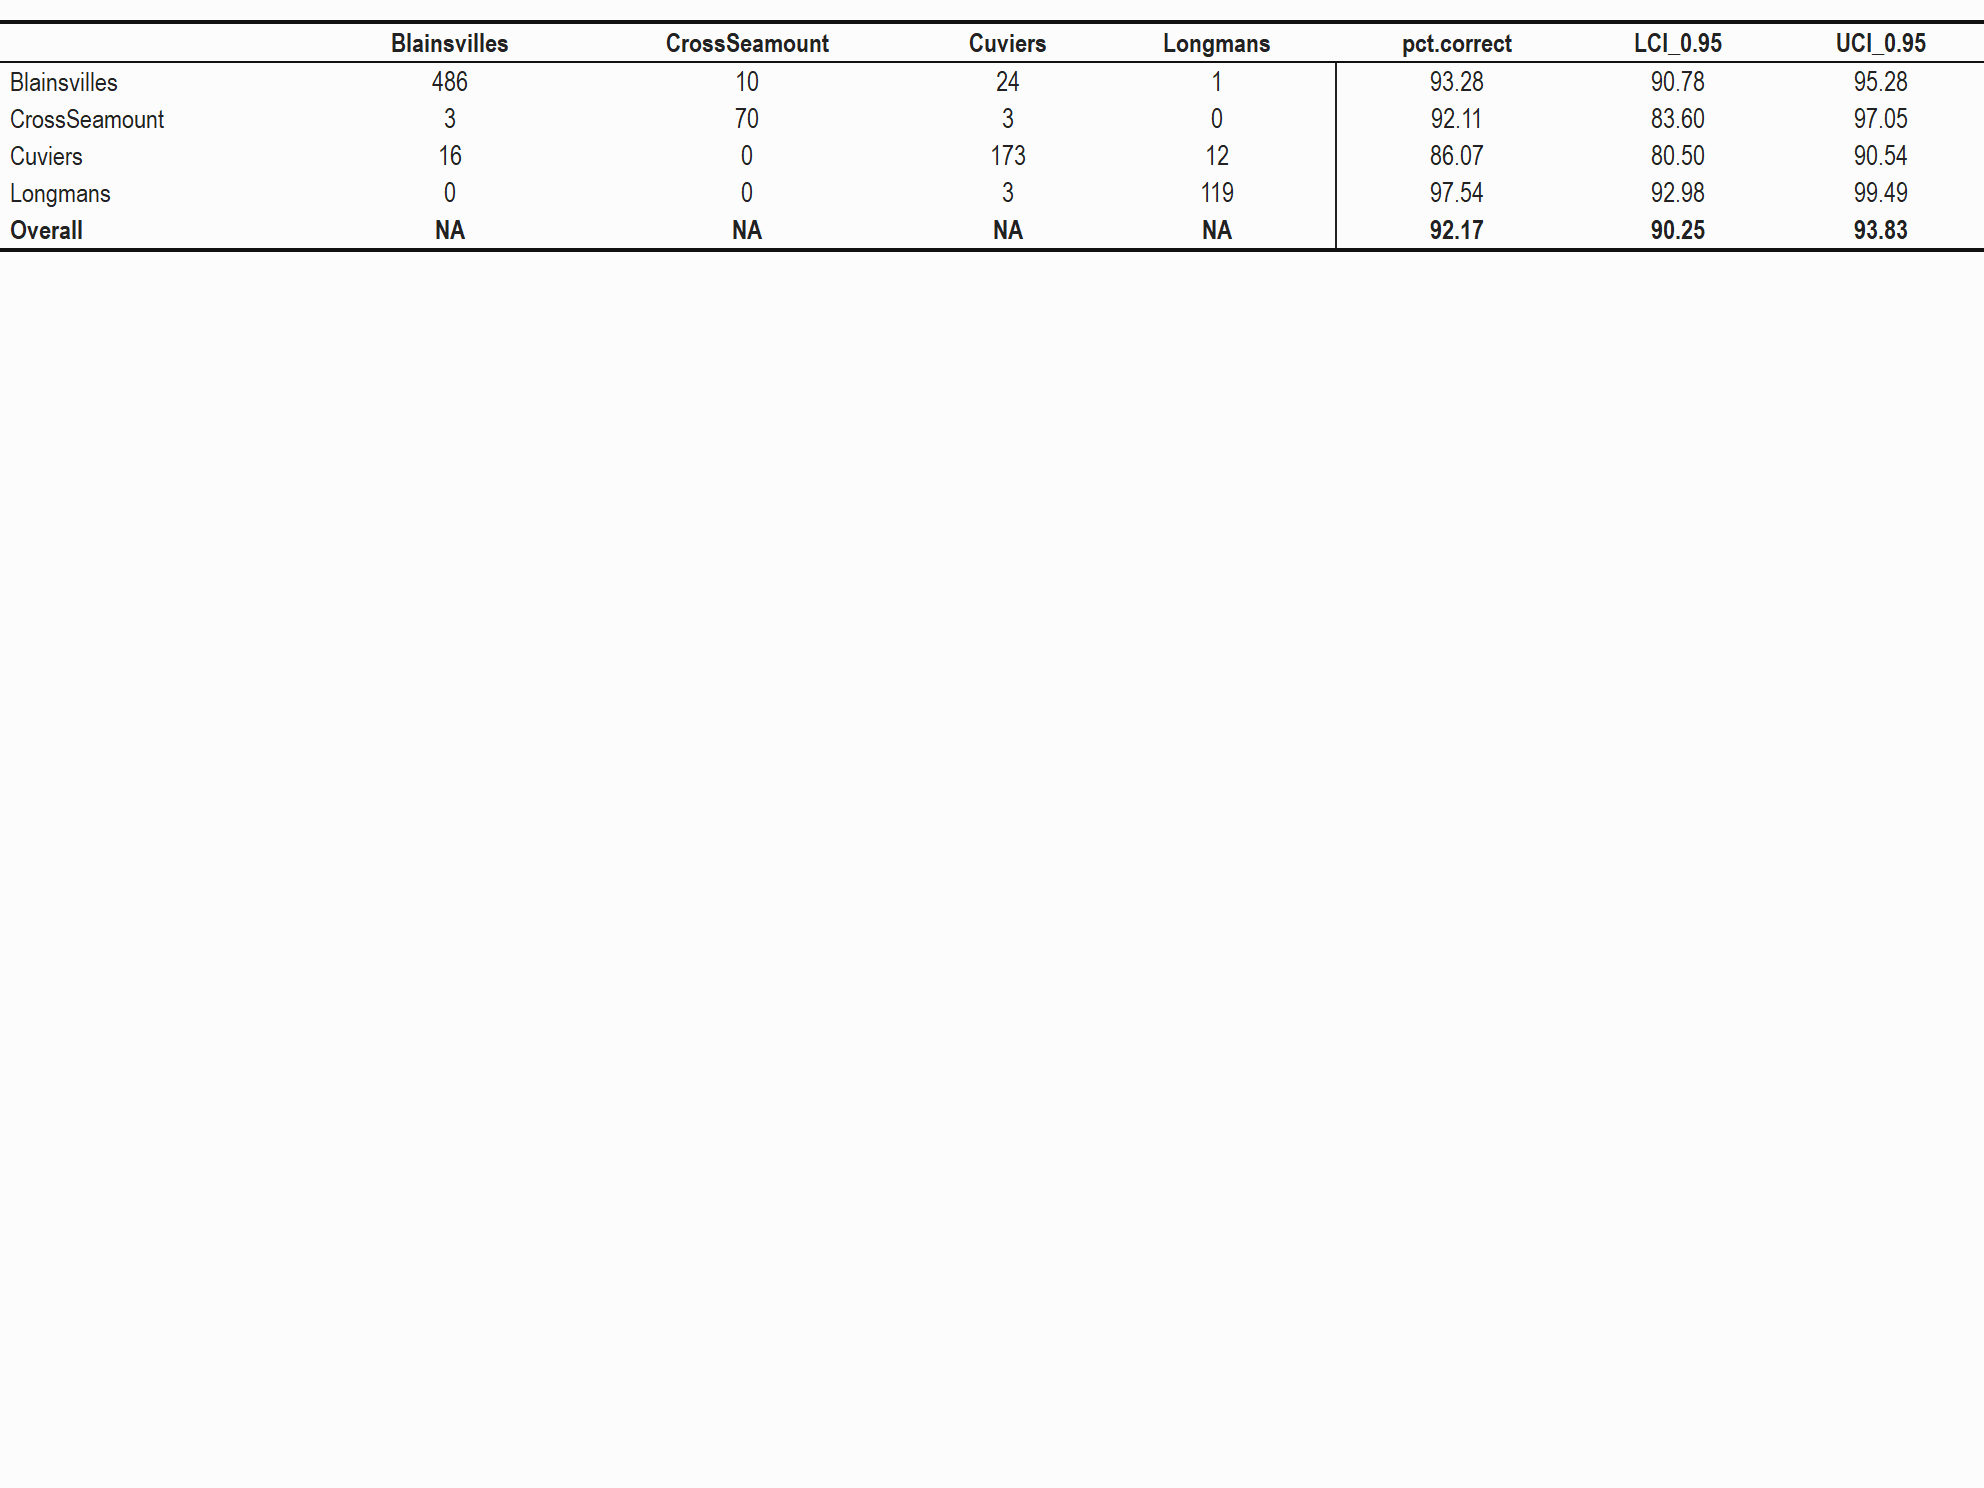
\includegraphics{../hawaii/banter_model_hawaii_confuseMatrix.png}

  }

  \caption{\label{fig-a}Fig.1}

  \end{figure}
\item
  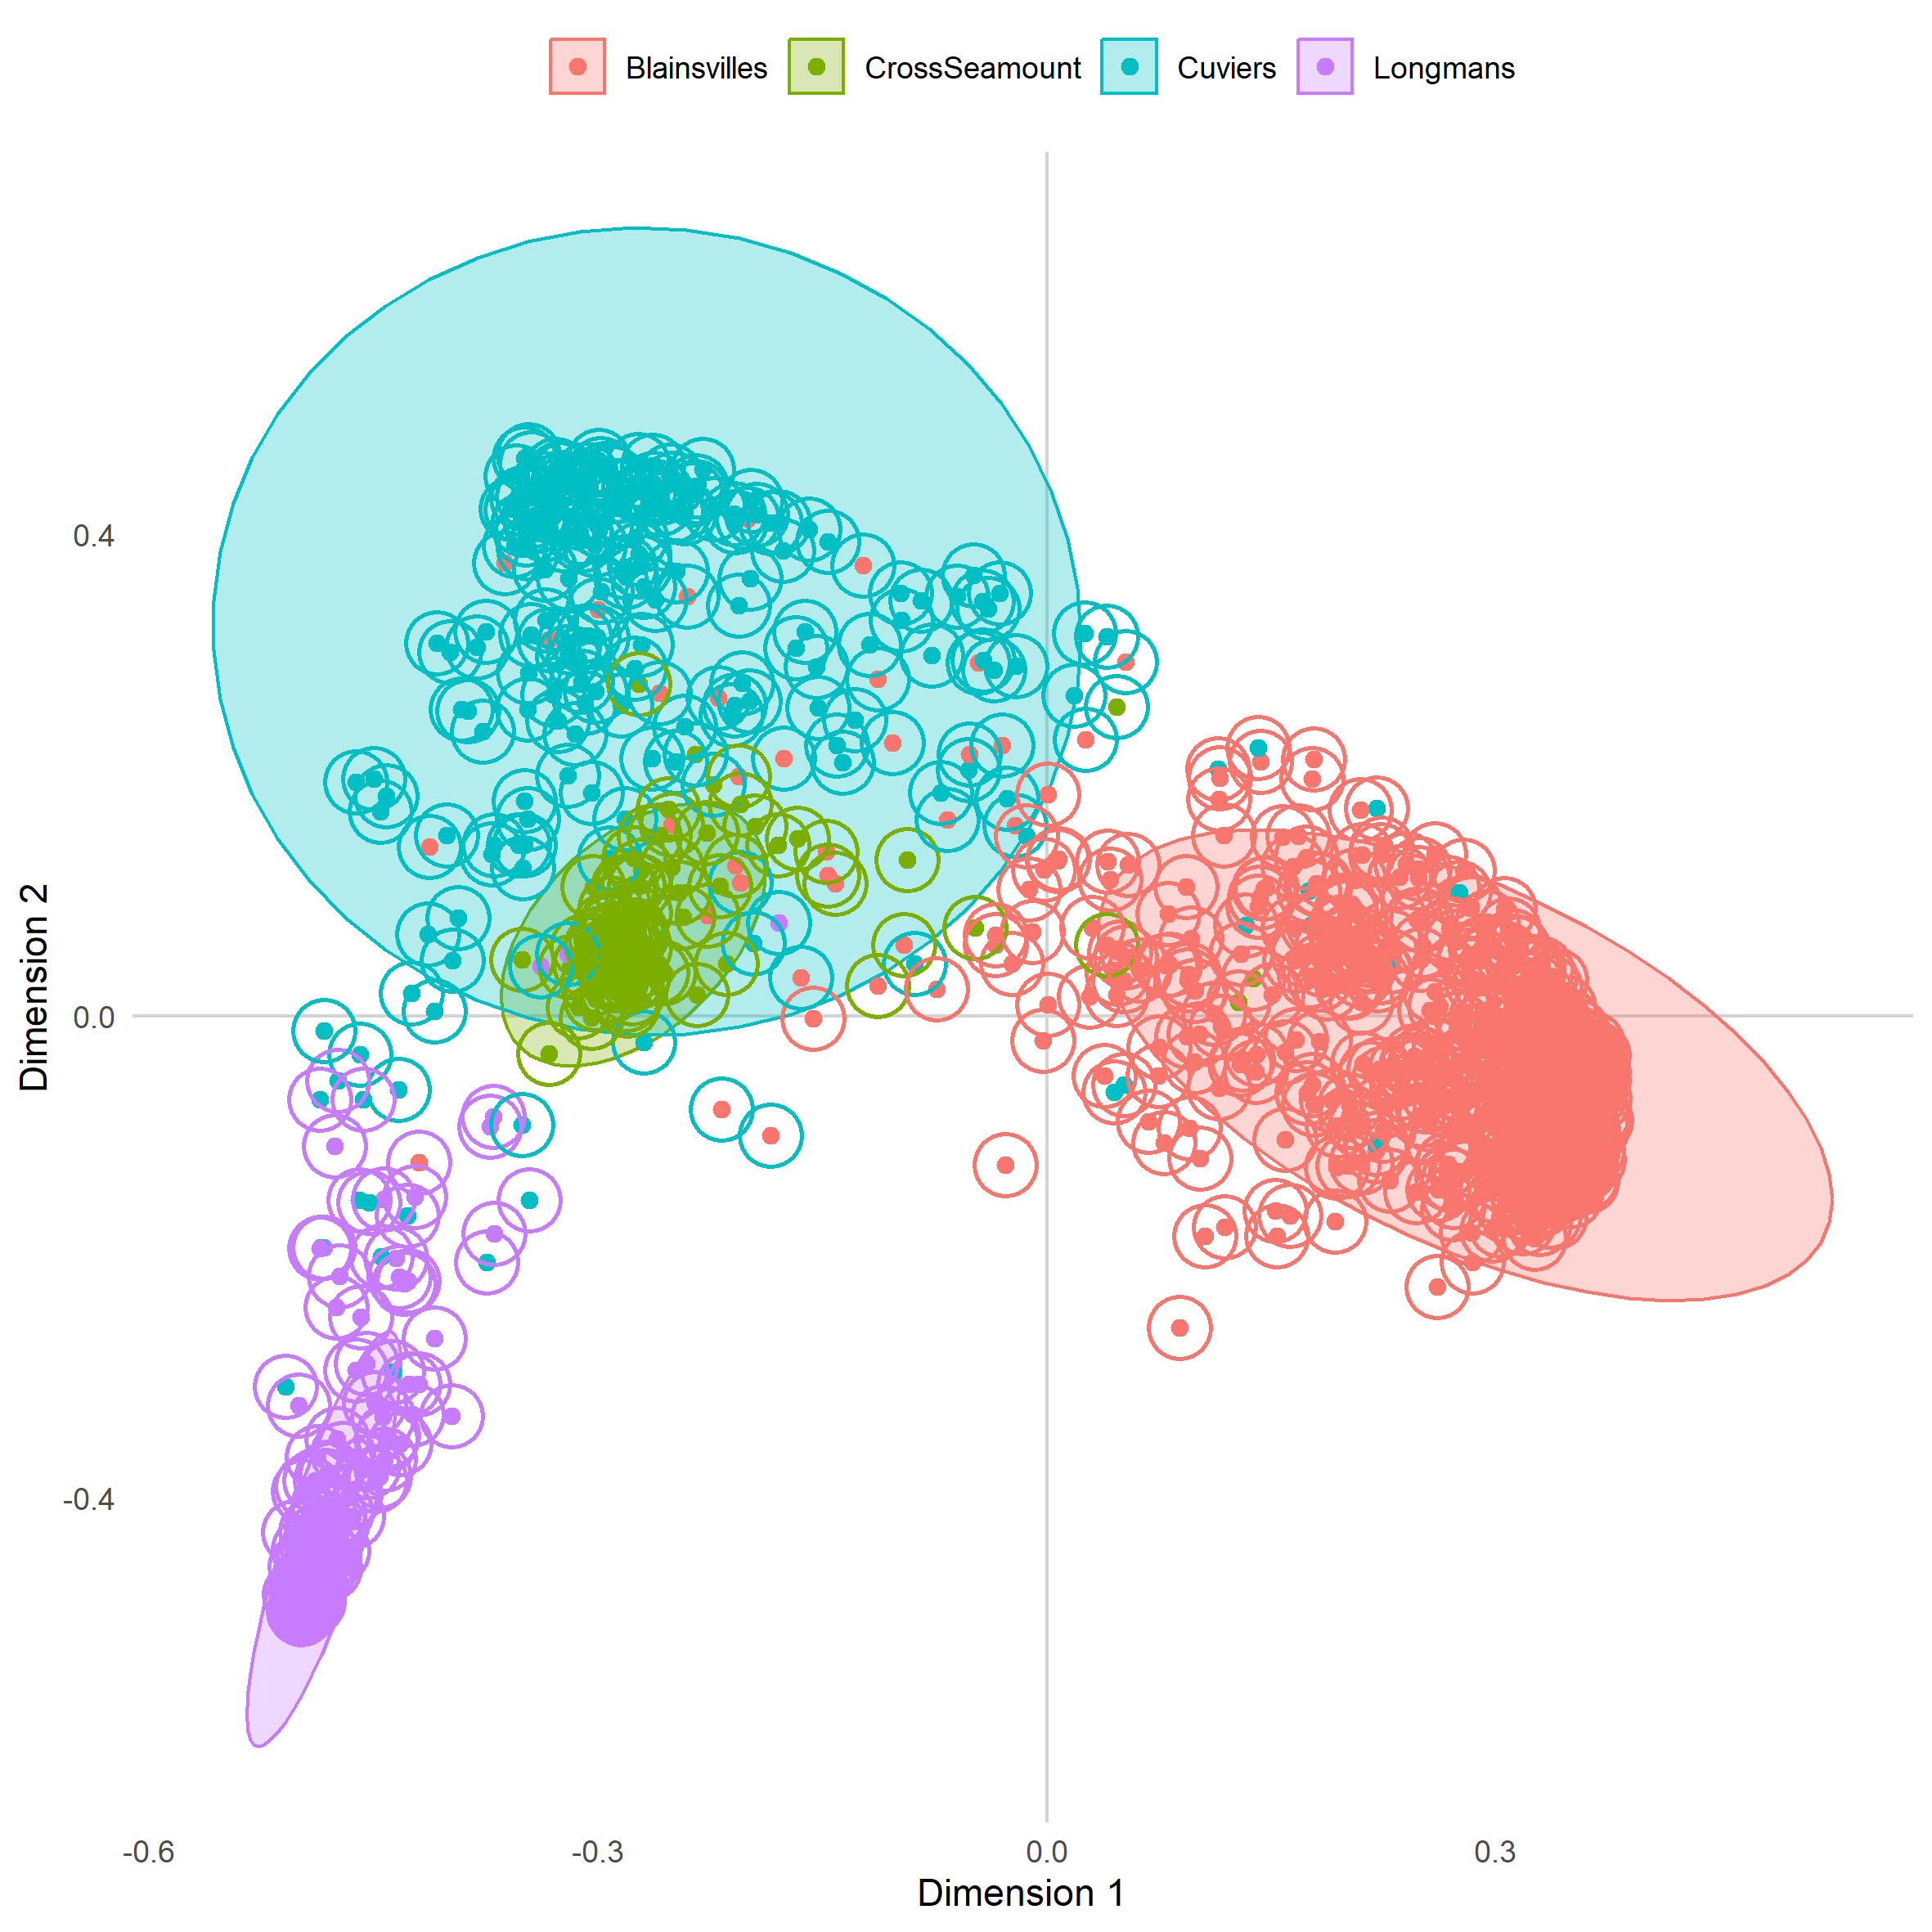
\includegraphics{../hawaii/banter_model_hawaii_proximity.png} :::
\item
  \begin{figure}

  {\centering 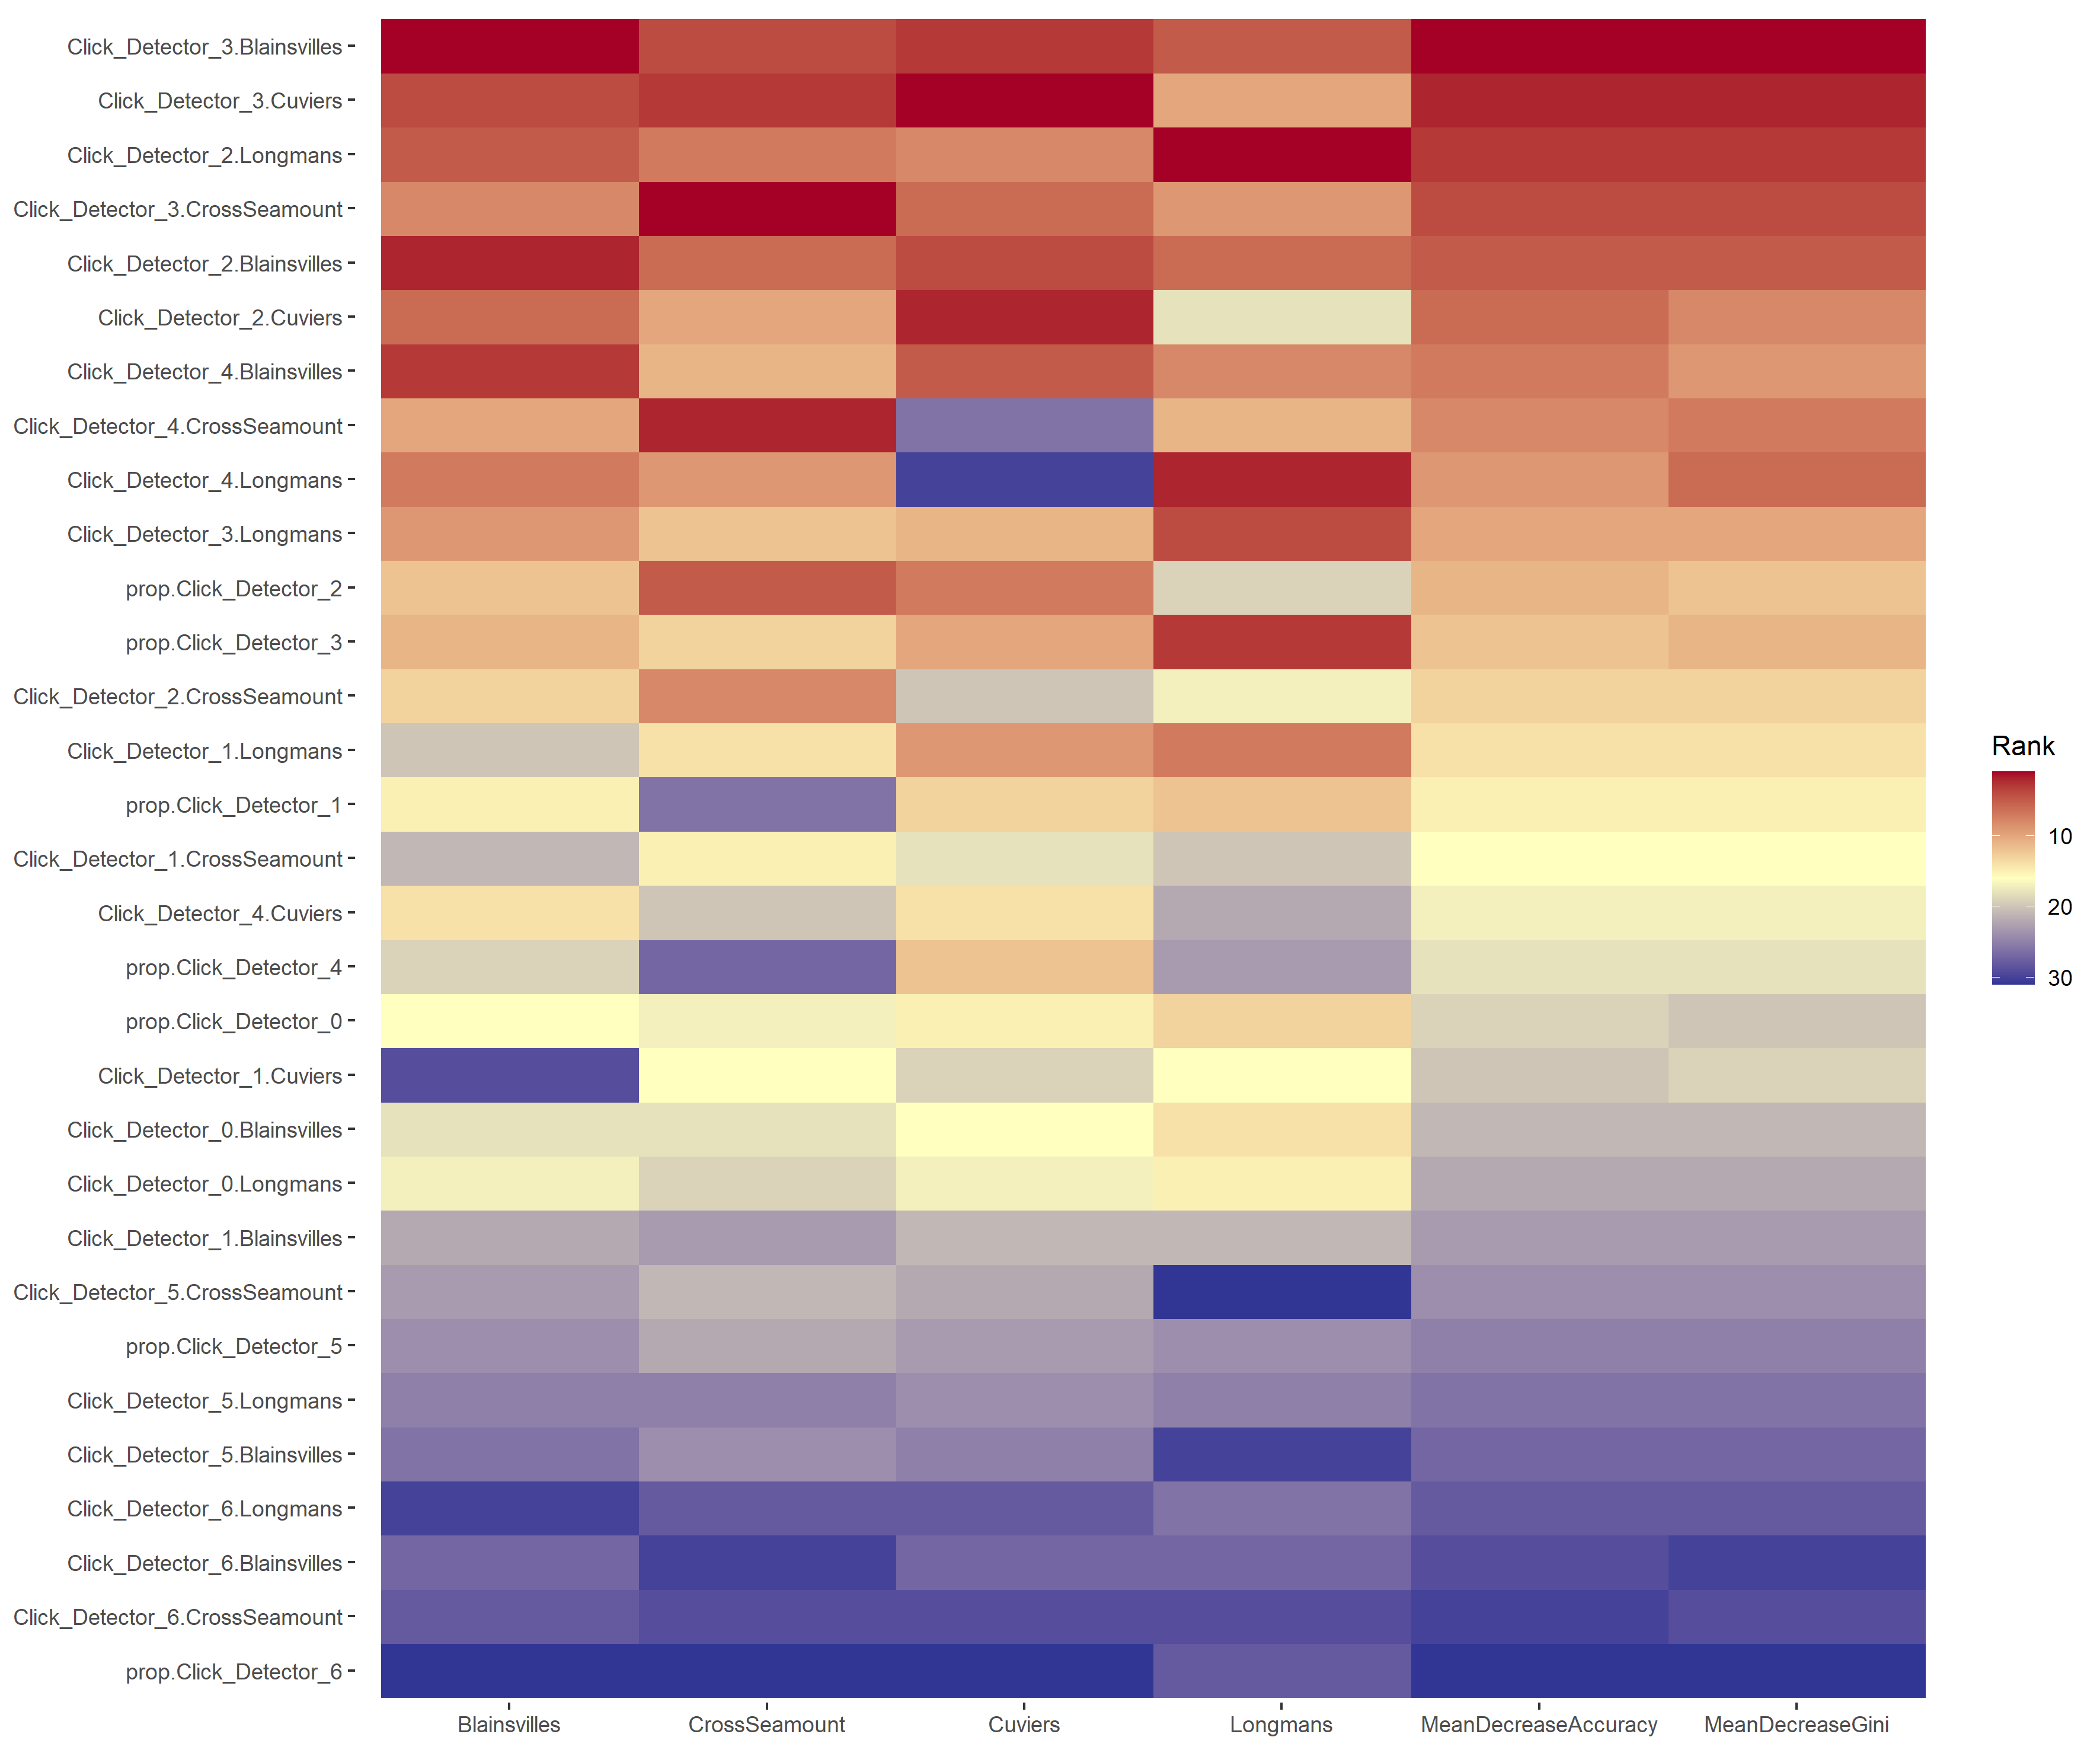
\includegraphics{../hawaii/banter_model_hawaii_importance.png}

  }

  \caption{Fig.1}

  \end{figure}
\item
  \begin{figure}

  {\centering 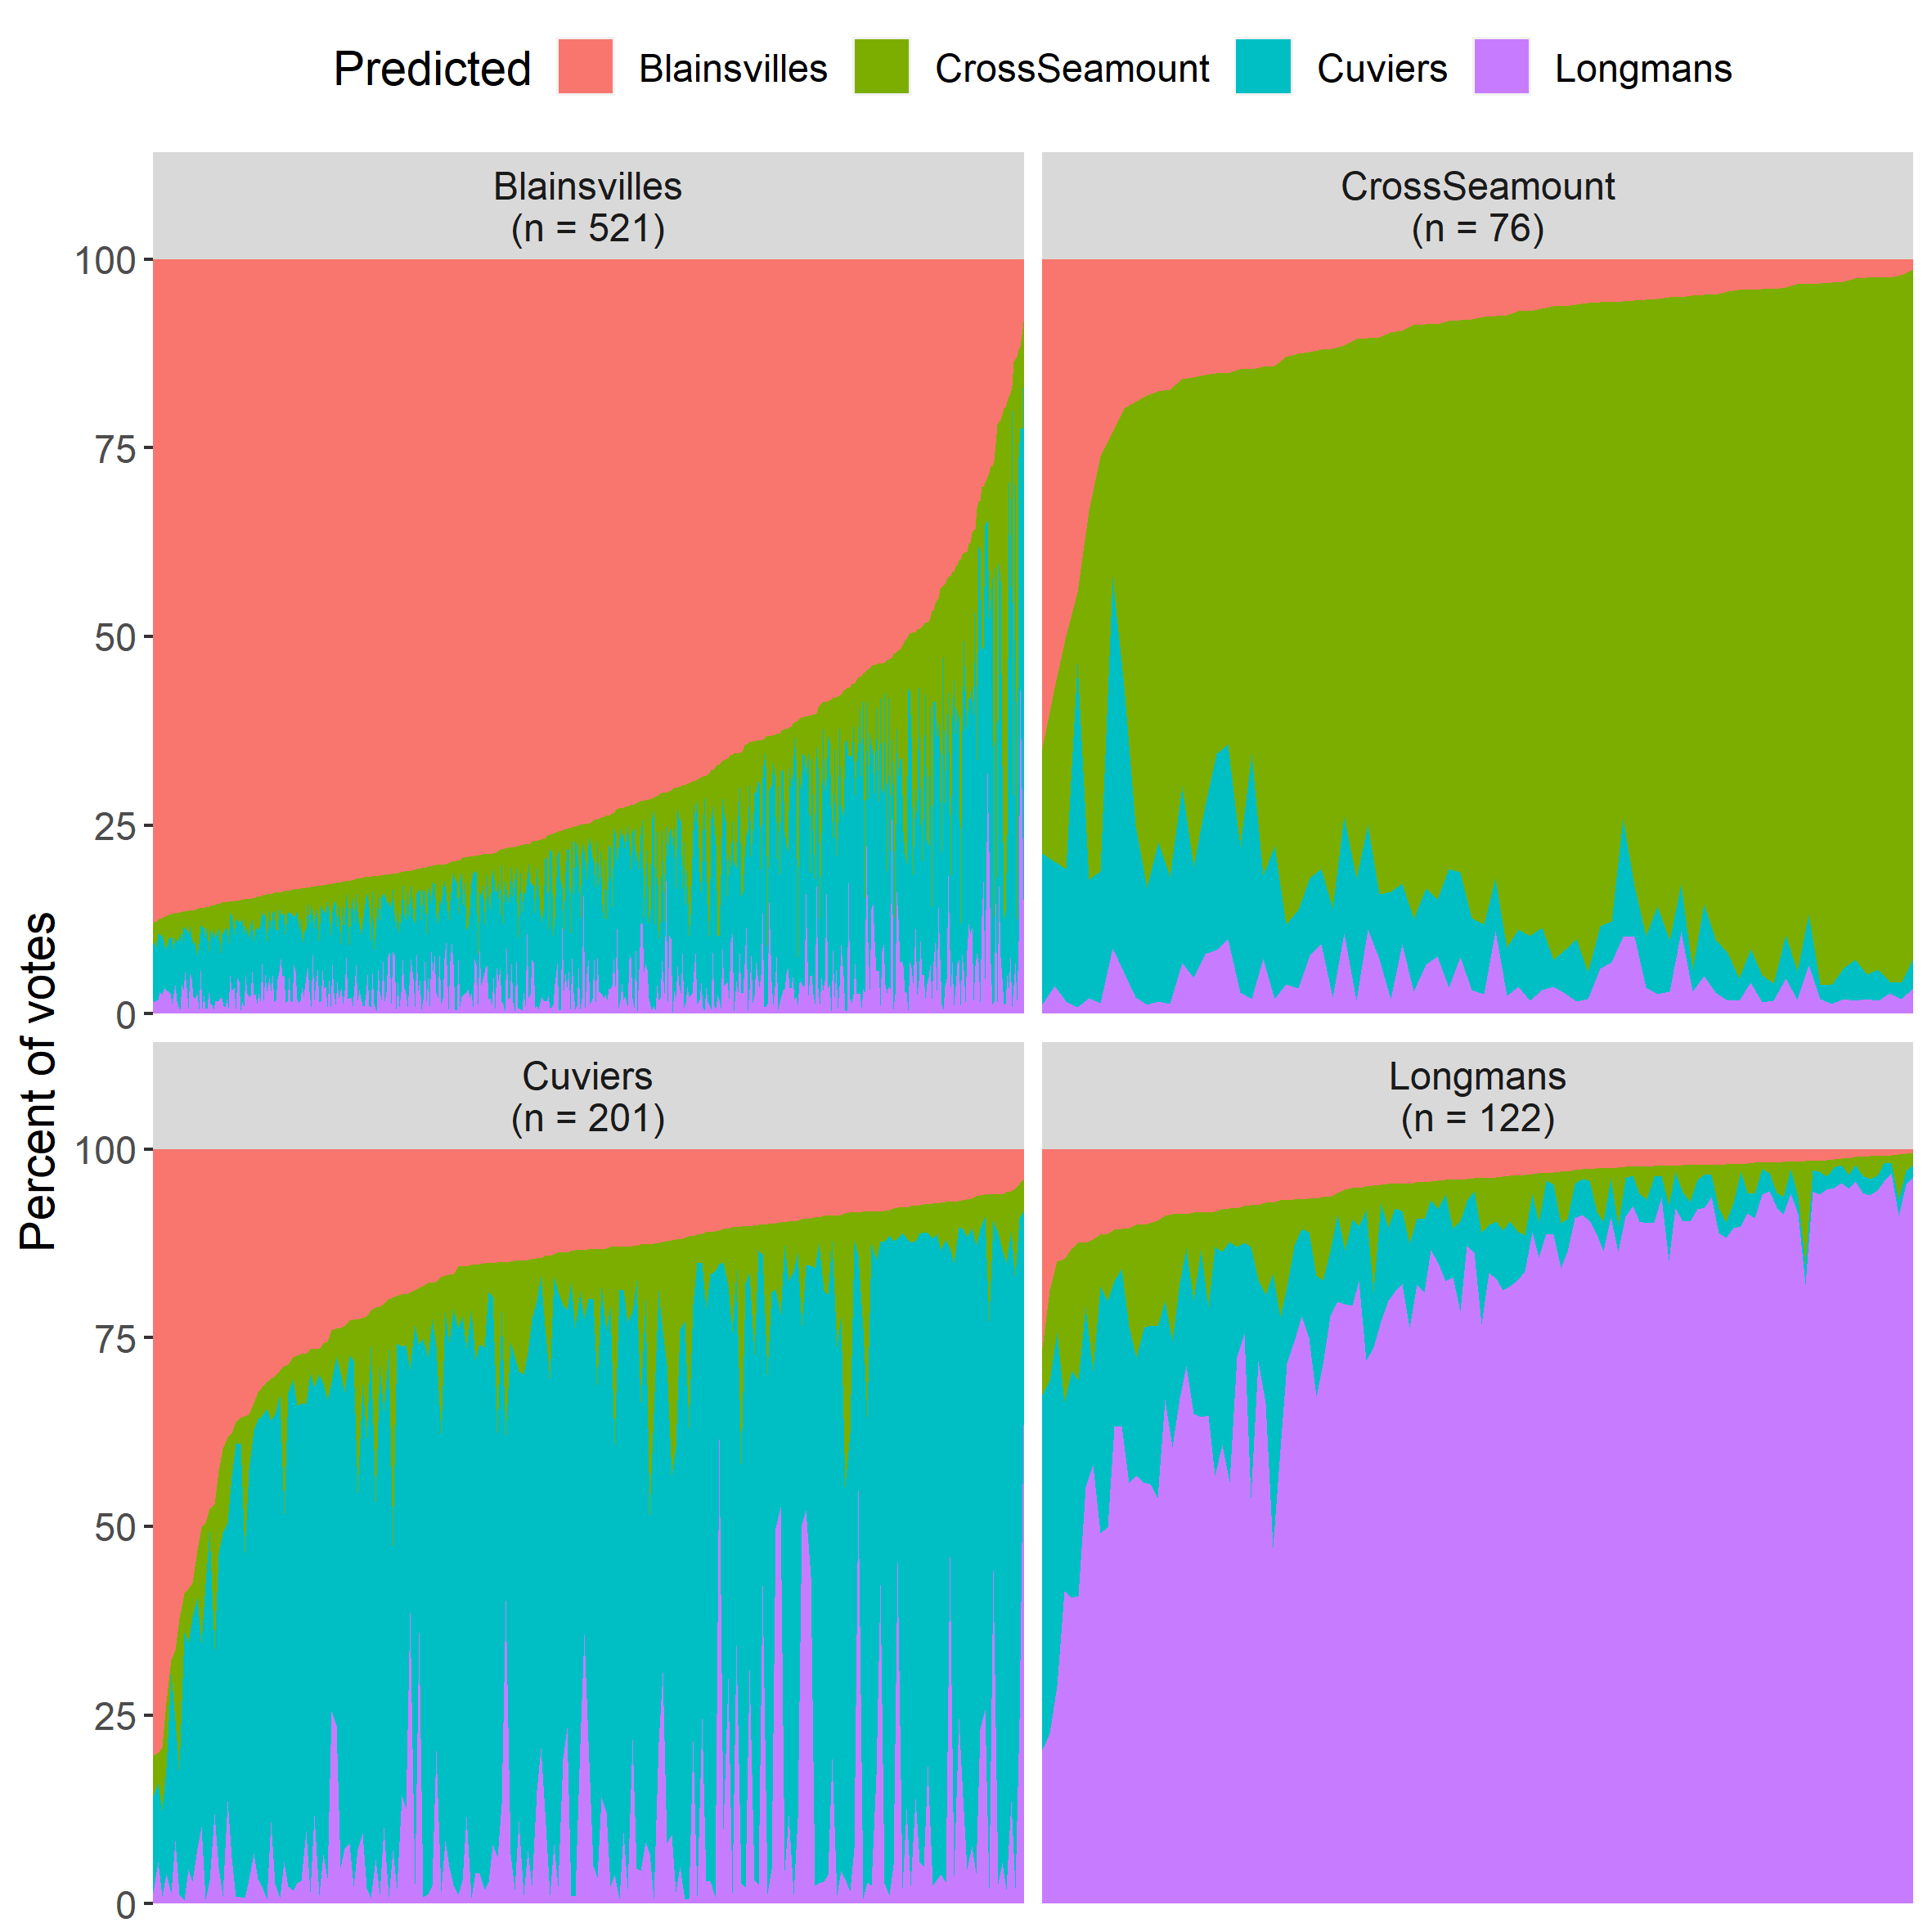
\includegraphics{../hawaii/banter_model_hawaii_votes.png}

  }

  \caption{Fig.1}

  \end{figure}
\end{enumerate}

}

\end{minipage}%

\end{figure}

{[}Insert Figure 3{]}{[}Figure 3. BANTER classification results from the
Hawaii dataset. Confusion matrix (a) provides the percent correct
classification for each species (pct.correct), lower confidence
intervals (LCI\_0.95), upper confidence intervals (UCI\_0.95), priors
(expected error rate). Proximity plot (b) for species events from BANTER
model (central dot color represents true species identity; color of
circle surrounding dot represents BANTER species classification). Heat
map (c) for ranks of variable importance for each species; colors scale
from most important predictors (dark red) to least important predictors
(dark blue). Vote Plot (d) shows the vote distribution for each event
(vertical slice) for each species; distribution of votes by species is
shown by their representative color. Species codes include Cross
Seamount beaked whale (BWC), Longman's beaked whale (IP), Blainsville's
beaked whale (MD) and Cuvier's beaked whale (ZC).

There are clear distinctions in the primary features used to classify
three of the four species as shown in the Proximity Plot (Fig. 3b) which
shows the classification results based on the two most `important'
predictors. Distinctive clusters based on the two most important
features can be found for Longman's (IP), Blainsville's (MD), and
Cuvier's beaked whales (ZC), and there is overlap in the feature space
of the clusters for Cuvier's and Cross Seamount beaked whales (BWC).
This overlap is resolved with different features for ZC
(3\textsuperscript{rd}, 7\textsuperscript{th} in Fig. 3c heat map) and
BWC (5\textsuperscript{th}, 8\textsuperscript{th} feature in heat map),
as evidence in the low misclassification rates for these species (Fig.
3a confusion matrix). The plot votes graph (Fig. 3d) show complicated
results with variation in the proportion of trees that correctly
classified the species for each event.

\hypertarget{eastern-pacific}{%
\subsection{Eastern Pacific}\label{eastern-pacific}}

The EPacific dataset consisted of 25 drifting recording buoys (20
stations plus 5 seamount experiment drifts) deployed off the west coast
of the United States ((J. Keating et al. 2018a)); species included
Baird's beaked whale (n=91), Unidentified Beaked Whale `BW43' (n=11),
Stejneger's beaked whale (n=41) and Cuvier's beaked whale (n=1,332).
BANTER classification trials included (1) echolocation clicks (EC) and
(2) echolocation clicks and ICI (EC\_ICI).

The best model considered the echolocation clicks and the ICI values
(Detector Model: sampsize = 5, ntrees = 30,000; BANTER model: sampsize =
4, ntree = 200,000) and provided an overall correct classification rate
of 93.7\% for all four species. Classification scores ranged from a low
of 93.2\% (Cuvier's beaked whale) to 100\% (BW43, Fig. 4a). All
classification results were greater than the expected error rate (Prior
in Fig. 4a). Results from the EC\_ICI model are presented here; complete
results can be found in supplementary materials (Supplement Figs. 5-7).

{[}Insert Figure 4{]}{[}Figure 4. BANTER classification results from the
EPacific dataset. Confusion matrix (a) provides the percent correct
classification for each species (pct.correct), lower confidence
intervals (LCI\_0.95), upper confidence intervals (UCI\_0.95), priors
(expected error rate).~ Proximity plot (b) for species events from
BANTER model (central dot color represents true species identity; color
of circle surrounding dot represents BANTER species classification).
Heat map (c) for ranks of variable importance for each species; colors
scale from most important predictors (dark red) to least important
predictors (dark blue). Vote Plot (d) shows the vote distribution for
each event (vertical slice) for each species; distribution of votes by
species is shown by their representative color. Species codes include
Baird's beaked whale (BB), unidentified beaked whale (BW43), Stejneger's
beaked whale (MS) and Cuvier's beaked whale (ZC).{]}

There are clear distinctions in the primary features used to classify
the species as shown in the Proximity Plot (Fig. 4b) which shows the
classification results based on the two most `important' predictors. The
species each form distinctive clusters based on these two features;
however, many events fall outside these distinct bounds (detections
shown in area between species classification clusters). Both BB and BW43
relied on a wide range of variables for classification (Fig. 4c heat
map). The plot votes (Fig. 4d) show strong classification results for
most events of most species.

\hypertarget{discussion}{%
\section{Discussion}\label{discussion}}

The results for the four study areas varied from a low of 86.9\% correct
classification in the SAtlantic dataset to a high of 100\% correct
classification in the NAtlantic dataset. All species in all datasets had
classifications rates well above those expected by chance; however
Cuvier's (SAtlantic, Hawaii), BWC (Hawaii), and Blainsville's beaked
whales (Hawaii) had classification rates below 90\%. There were
insufficient sample sizes of Gervais to include in the NAtlantic
dataset.

Several of our datasets included very low sample sizes for some species;
however, low sample sizes did not always result in low classification
scores. In the Atlantic dataset, Sowerby's beaked whale was consistently
correctly classified in both models (NAtlantic and SAtlantic); however,
while the plot votes showed very strong classification strength in the
NAtlantic, the classification strength (represented by the number of
trees that voted for the correct classification) was poor in the
SAtlantic study area.This is likely due to both a small sample size of
Sowerby's detected in the S. study area (n=2) combined with the small
sampsize used in the BANTER model. In general, larger sample sizes
should lead to improved overall classification results, and improved
strength of these classification results (as identified by plot vote
graph).

While some species have distinctive differences in their click
characteristics that lead to strong classification despite small sample
sizes (e.g.~Sowerby's beaked whales in NAtlantic); other species, such
as Cuvier's beaked whales, have significant variation in their click
measurements. ~For species with high variability in the predictor
variables and an overlap in the range of these variables with other
species, a large sample size is required to describe the true
variability of these call measurements. Even with reasonably large
sample sizes, the classification may suffer (e.g, SAtlantic Cuvier's
beaked whale = 74\%). We found by increasing the sampsize in BANTER, we
could increase the classification rate for this species in this area to
(97\%, see Supplement Fig.3); however, this resulted in the loss of
Sowerby's beaked whale in the final model. So, an increased sample size
in Sowerby's would likely lead to increased classification results for
other species in the model.

Previous application of BANTER to dolphin species in the California
Current found that large sample sizes could result in strong
classification of species where experienced acousticians are unable to
differentiate species (long-beaked and short-beaked common dolphins,
(Rankin et al. 2017c)). This suggests that large increases in sample
size may improve classification results for Cuvier's beaked whales.

Researchers have noted several `types' of click characteristics for
Cuvier's beaked whales (ADA, pers. comm) which may be related to
variability in the propagation environment, different animal behaviors,
gender or age classes, or acoustic populations. Future work should
examine if these Cuvier's beaked whale events can be clustered in an
objective and stable manner; if so, then these can be input into BANTER
models as separate types of Cuvier's beaked whales. We recommend caution
in this approach- this should only be considered if there is reasonable
evidence that these different groups represent authentic cluster. We do
not recommend segregation of misclassified subgroups simply to improve
classification scores.

Gervais' and True's beaked whales have similar click characteristics
that make them difficult to differentiate, and require considerable
expertise to classify manually, using a variety of available visuals and
metrics ((DeAngelis et al. 2018c)). Our results suggest that BANTER may
serve as an efficient and effective means of classifying and
differentiating these two species. Despite modest sample sizes, Gervais'
and True's beaked whales showed high classification scores (95.6\% and
100\%, respectively). Unfortunately, we were unable to combine the N and
S Atlantic datasets (which would increase sample sizes of True's beaked
whales) due to differences in hydrophone characteristics that result in
differences in call measures. Calibration of signals (to make them
comparable) may allow for combining datasets to improve sample sizes.

For the SAtlantic models, ICI was found to be an important predictor for
many species {[}\emph{talk about the 1 change in sowerby's when the ICI
was added- do you think it was because of an error in ICI?}{]} . For
Hawaii and the EPacific, however, we found that adding ICI into the
BANTER classifier did not improve final classification results. The
differences here are likely due to different analysis methods for
identifying events. Beaked whale events were defined by encounter time
for both the Hawaii and EPacific data, which were collected using
drifting acoustic recorders where animals could not be localized. The
Atlantic data were collected using a towed hydrophone array with
localization capabilities. Each event was defined as an individual click
train, so ICI for these events more likely represented true ICI, and was
found to be more informative. (Baumann-Pickering et al. 2013a) showed an
overlap in the ICI between Cuvier's and Blainsville's beaked whales, but
a strong difference in ICI between these species and BWC. Likewise,
(Baumann-Pickering et al. 2013a) found a difference in ICI between
Baird's beaked whales and Cuvier's beaked whales. Subdividing click
trains in PAMGuard is time consuming, but alternative options include
consideration of the PAMGuard click train detector module in BANTER, or
by developing a similar function in R to apply to events. Integration of
ICI from individual click trains may serve to improve classification
results for some species in Hawaii and EPacific.

Gervais were eliminated from the NAtlantic BANTER model due to low
sample size (n=2); results were extremely poor when they were included
in the model. Analysis notes indicate uncertainty in manual species
classification on one of the two events in this dataset. While small
sample size can at times provide good classification scores, as we found
in Sowerby's beaked whale in this SAtlantic dataset, they can be
devastating if there are inaccuracies in the training data. These two
examples of small sample sizes highlights a conflict in preferred
protocol. Ideally, (1) all \uline{species} would be included in a
classification model, so as to better represent the local species
diversity, (2) all \uline{events} would ideally be included in the
classification model, so as to better represent the variability found in
the area, and (3) only confident `ground truth' classifications would be
considered in the training model. Unfortunately, in species where
identity must be determined based on call characteristics (rather than
visual confirmation of species identity in the field), it can sometimes
be difficult to confidently determine species identity when calls are
highly variable and do not include at least one call that provides high
confidence of species identity. In the case of beaked whales, we
recommend that training data include a reasonable level of confidence
for inclusion. When sample sizes are low, such as in these cases, it may
be wise to consider the strength of the classifications when including
them for model training (as we have done here). An alternative is to
require agreement from multiple analysts, as provided by the EPacific
datasets. This concern about accurate labeling of training data is
further complicated by the potential existence of species that have not
yet been identified. For example, (cite jays new paper) recently
discovered what appears to be a new species of beaked whale off Baja
California, Mexico; this putative new species may have been detected but
misclassified in other datasets (including the EPacific data presented
here).

While BANTER provides an efficient and consistent approach to
classification, there are significant limitations that must be
considered. BANTER is a supervised machine learning tool and requires
reliable training data for success. Training data should consist of
labels with strong confidence in species identify (ideally determined by
agreement from more than one analyst) and sample sizes should be large
enough to explain the natural variability in the data. In fact,
consideration of the strength of classification scores may help identify
cases where the training data were of poor quality, or where there may
be evidence to identify different acoustic populations or behavior
states.

The workflow presented here provides a highly automated approach to
detection of acoustic events (PAMGuard), integration of environmental
data (PAMpal) and acoustic event classification (BANTER). These methods
significantly reduce manual analysis, provide more consistent
classification results with fewer biases, and provide an estimate of
classification error.~ The greatest improvement to classification
results for beaked whales would likely result from improved sample sizes
and examination of individual click trains in measuring ICI.
Consideration of additional detectors (e.g.~matched filter detector,
click train detector) or additional environmental variables may further
improve classification results. These highly automated methods may allow
for analysis of data across large spatial and temporal scales to address
large ecological and population level questions.

\hypertarget{acknowledgements}{%
\section{Acknowledgements}\label{acknowledgements}}

The authors would like to acknowledge the large number of scientists and
shipboard crew who were responsible for data collection during multiple
large scale studies. Funding for data collection and analysis were
provided by U.S. Navy, Bureau of Ocean Energy Management, and the
National Oceanographic and Atmospheric Administration. The manuscript
was improved thanks to reviews from {[}XXXX{]}.

Here are two sample references: (\textbf{Feynman1963118?})
(\textbf{Dirac1953888?}).

By default, natbib will be used with the \texttt{authoryear} style, set
in \texttt{classoption} variable in YAML. You can sets extra options
with \texttt{natbiboptions} variable in YAML header. Example

\begin{verbatim}
natbiboptions: longnamesfirst,angle,semicolon
\end{verbatim}

There are various more specific bibliography styles available at
\url{https://support.stmdocs.in/wiki/index.php?title=Model-wise_bibliographic_style_files}.
To use one of these, add it in the header using, for example,
\texttt{biblio-style:\ model1-num-names}.

\hypertarget{using-csl}{%
\subsection{Using CSL}\label{using-csl}}

If \texttt{cite-method} is set to \texttt{citeproc} in
\texttt{elsevier\_article()}, then pandoc is used for citations instead
of \texttt{natbib}. In this case, the \texttt{csl} option is used to
format the references. By default, this template will provide an
appropriate style, but alternative \texttt{csl} files are available from
\url{https://www.zotero.org/styles?q=elsevier}. These can be downloaded
and stored locally, or the url can be used as in the example header.

\hypertarget{figures-and-tables}{%
\section{Figures and tables}\label{figures-and-tables}}

Figure~\ref{fig-meaningless} is generated using an R chunk.

\begin{figure}

{\centering 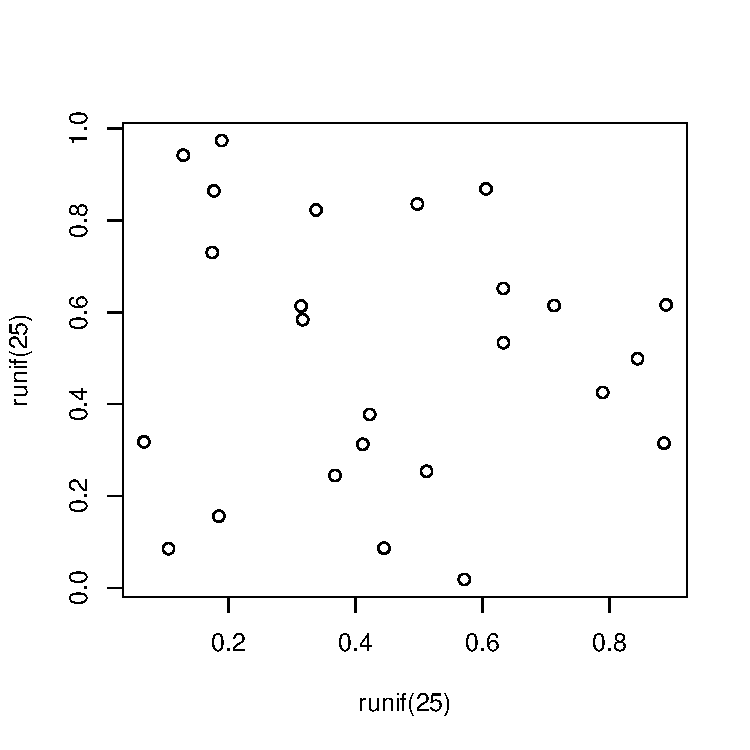
\includegraphics[width=0.5\textwidth,height=\textheight]{manuscript_files/figure-pdf/fig-meaningless-1.pdf}

}

\caption{\label{fig-meaningless}A meaningless scatterplot}

\end{figure}

\hypertarget{tables-coming-from-r}{%
\section{Tables coming from R}\label{tables-coming-from-r}}

Tables can also be generated using R chunks, as shown in
Table~\ref{tbl-simple} example.

\begin{Shaded}
\begin{Highlighting}[]
\NormalTok{knitr}\SpecialCharTok{::}\FunctionTok{kable}\NormalTok{(}\FunctionTok{head}\NormalTok{(mtcars)[,}\DecValTok{1}\SpecialCharTok{:}\DecValTok{4}\NormalTok{])}
\end{Highlighting}
\end{Shaded}

\hypertarget{tbl-simple}{}
\begin{longtable}[]{@{}lrrrr@{}}
\caption{\label{tbl-simple}Caption centered above table}\tabularnewline
\toprule()
& mpg & cyl & disp & hp \\
\midrule()
\endfirsthead
\toprule()
& mpg & cyl & disp & hp \\
\midrule()
\endhead
Mazda RX4 & 21.0 & 6 & 160 & 110 \\
Mazda RX4 Wag & 21.0 & 6 & 160 & 110 \\
Datsun 710 & 22.8 & 4 & 108 & 93 \\
Hornet 4 Drive & 21.4 & 6 & 258 & 110 \\
Hornet Sportabout & 18.7 & 8 & 360 & 175 \\
Valiant & 18.1 & 6 & 225 & 105 \\
\bottomrule()
\end{longtable}

\hypertarget{references}{%
\section*{References}\label{references}}
\addcontentsline{toc}{section}{References}

\hypertarget{refs}{}
\begin{CSLReferences}{1}{0}
\leavevmode\vadjust pre{\hypertarget{ref-archer2022}{}}%
Archer, Frederick. 2022a. \emph{Banter: BioAcoustic eveNT classifiER}.
\url{https://cran.r-project.org/web/packages/banter/index.html}.

\leavevmode\vadjust pre{\hypertarget{ref-archer2022a}{}}%
---------. 2022b. \emph{rfPermute: Estimate Permutation p-Values for
Random Forest Importance Metrics}.
\url{https://cran.r-project.org/web/packages/rfPermute/index.html}.

\leavevmode\vadjust pre{\hypertarget{ref-barlow2022}{}}%
Barlow, Jay, Jeffrey E. Moore, Jennifer L. K. McCullough, and Emily T.
Griffiths. 2022. {``Acoustic-Based Estimates of Cuvier's Beaked Whale
(Ziphius Cavirostris) Density and Abundance Along the U.S. West Coast
from Drifting Hydrophone Recorders.''} \emph{Marine Mammal Science} 38
(2): 517--38. \url{https://doi.org/10.1111/mms.12872}.

\leavevmode\vadjust pre{\hypertarget{ref-baumann-pickering2013}{}}%
Baumann-Pickering, Simone, Mark A. McDonald, Anne E. Simonis, Alba
Solsona Berga, Karlina P. B. Merkens, Erin M. Oleson, Marie A. Roch, et
al. 2013a. {``Species-Specific Beaked Whale Echolocation Signals.''}
\emph{The Journal of the Acoustical Society of America} 134 (3):
2293--2301. \url{https://doi.org/10.1121/1.4817832}.

\leavevmode\vadjust pre{\hypertarget{ref-baumann-pickering2013a}{}}%
---------, et al. 2013b. {``Species-Specific Beaked Whale Echolocation
Signals.''} \emph{The Journal of the Acoustical Society of America} 134
(3): 2293--2301. \url{https://doi.org/10.1121/1.4817832}.

\leavevmode\vadjust pre{\hypertarget{ref-baumann-pickering2014}{}}%
Baumann-Pickering, Simone, Marie A. Roch, Robert L. Brownell Jr, Anne E.
Simonis, Mark A. McDonald, Alba Solsona-Berga, Erin M. Oleson, Sean M.
Wiggins, and John A. Hildebrand. 2014. {``Spatio-Temporal Patterns of
Beaked Whale Echolocation Signals in the North Pacific.''} \emph{PLOS
ONE} 9 (1): e86072. \url{https://doi.org/10.1371/journal.pone.0086072}.

\leavevmode\vadjust pre{\hypertarget{ref-bittle2013}{}}%
Bittle, Michael, and Alec Duncan. 2013. {``A Review of Current Marine
Mammal Detection and Classification Algorithms for Use in Automated
Passive Acoustic Monitoring.''} 8.

\leavevmode\vadjust pre{\hypertarget{ref-deangelis2018}{}}%
DeAngelis, Annamaria Izzi, Joy E. Stanistreet, Simone Baumann-Pickering,
and Danielle M. Cholewiak. 2018b. {``A Description of Echolocation
Clicks Recorded in the Presence of True's Beaked Whale (Mesoplodon
Mirus).''} \emph{The Journal of the Acoustical Society of America} 144
(5): 2691--2700. \url{https://doi.org/10.1121/1.5067379}.

\leavevmode\vadjust pre{\hypertarget{ref-deangelis2018a}{}}%
---------. 2018c. {``A Description of Echolocation Clicks Recorded in
the Presence of True's Beaked Whale (Mesoplodon Mirus).''} \emph{The
Journal of the Acoustical Society of America} 144 (5): 2691--2700.
\url{https://doi.org/10.1121/1.5067379}.

\leavevmode\vadjust pre{\hypertarget{ref-deangelis2018b}{}}%
---------. 2018a. {``A Description of Echolocation Clicks Recorded in
the Presence of True's Beaked Whale (Mesoplodon Mirus).''} \emph{The
Journal of the Acoustical Society of America} 144 (5): 2691--2700.
\url{https://doi.org/10.1121/1.5067379}.

\leavevmode\vadjust pre{\hypertarget{ref-keating2013}{}}%
Keating, Jennifer L., and Jay Barlow. 2013a. {``Summary of PAMGuard
Beaked Whale Click Detectors and Classifiers Used During the 2012
Southern California Behavioral Response Study.''}

\leavevmode\vadjust pre{\hypertarget{ref-keating2013a}{}}%
---------. 2013b. {``Summary of PAMGuard Beaked Whale Click Detectors
and Classifiers Used During the 2012 Southern California Behavioral
Response Study.''}

\leavevmode\vadjust pre{\hypertarget{ref-keating2018}{}}%
Keating, Jennifer, Jay Barlow, Emily T. Griffiths, and Jeffrey E. Moore.
2018a. {``Passive Acoustics Survey of Cetacean Abundance Levels
(PASCAL-2016) Final Report.''}
\url{https://www.boem.gov/sites/default/files/environmental-stewardship/Environmental-Studies/Pacific-Region/Studies/BOEM-2018-025.pdf}.

\leavevmode\vadjust pre{\hypertarget{ref-keating2018a}{}}%
---------. 2018b. {``Passive Acoustics Survey of Cetacean Abundance
Levels (PASCAL-2016) Final Report.''}
\url{https://www.boem.gov/sites/default/files/environmental-stewardship/Environmental-Studies/Pacific-Region/Studies/BOEM-2018-025.pdf}.

\leavevmode\vadjust pre{\hypertarget{ref-macleod2018}{}}%
MacLeod, Colin D. 2018. {``Beaked Whales, Overview.''} In, edited by
Bernd Würsig, J. G. M. Thewissen, and Kit M. Kovacs, 80--83. Academic
Press. \url{https://doi.org/10.1016/B978-0-12-804327-1.00062-5}.

\leavevmode\vadjust pre{\hypertarget{ref-parijs2009}{}}%
Parijs, Sofie M. Van, Chris W. Clark, Renata S. Sousa-Lima, Susan E.
Parks, Shannon Rankin, Denise Risch, and Ilse C. Van Opzeeland. 2009.
{``Management and Research Applications of Real-Time and Archival
Passive Acoustic Sensors over Varying Temporal and Spatial Scales.''}
\emph{Marine Ecology Progress Series} 395 (December): 21--36.
\url{https://doi.org/10.3354/meps08123}.

\leavevmode\vadjust pre{\hypertarget{ref-rcoreteam2022}{}}%
R Core Team. 2022. \emph{R: A Language and Environment for Statistical
Computing}. Vienna, Austria: R Foundation for Statistical Computing.
\url{http://www.R-project.org/}.

\leavevmode\vadjust pre{\hypertarget{ref-rankin2021}{}}%
Rankin, Shannon, and Frederick Archer. 2021. {``BANTER: A User's Guide
to Acoustic Classification.''}
\url{https://taikisan21.github.io/PAMpal/banterGuide.html}.

\leavevmode\vadjust pre{\hypertarget{ref-rankin2017}{}}%
Rankin, Shannon, Frederick Archer, Jennifer L. Keating, Julie N. Oswald,
Michael Oswald, Alex Curtis, and Jay Barlow. 2017a. {``Acoustic
Classification of Dolphins in the California Current Using Whistles,
Echolocation Clicks, and Burst Pulses.''} \emph{Marine Mammal Science} 2
(33): 520--40. \url{https://doi.org/10.1111/mms.12381}.

\leavevmode\vadjust pre{\hypertarget{ref-rankin2017a}{}}%
---------. 2017b. {``Acoustic Classification of Dolphins in the
California Current Using Whistles, Echolocation Clicks, and Burst
Pulses.''} \emph{Marine Mammal Science} 2 (33): 520--40.
\url{https://doi.org/10.1111/mms.12381}.

\leavevmode\vadjust pre{\hypertarget{ref-rankin2017b}{}}%
---------. 2017c. {``Acoustic Classification of Dolphins in the
California Current Using Whistles, Echolocation Clicks, and Burst
Pulses.''} \emph{Marine Mammal Science} 2 (33): 520--40.
\url{https://doi.org/10.1111/mms.12381}.

\leavevmode\vadjust pre{\hypertarget{ref-rankin2005}{}}%
Rankin, Shannon, and Jay Barlow. 2005. {``Source of the North Pacific
{``}Boing{''} Sound Attributed to Minke Whales.''} \emph{The Journal of
the Acoustical Society of America} 118 (5): 3346--51.
\url{https://doi.org/10.1121/1.2046747}.

\leavevmode\vadjust pre{\hypertarget{ref-sakai2021}{}}%
Sakai, Taiki. 2021. \emph{PAMpal: Load and Process Passive Acoustic
Data}. \url{https://cran.r-project.org/web/packages/PAMpal/index.html}.

\leavevmode\vadjust pre{\hypertarget{ref-simonis2020}{}}%
Simonis, Anne E., Robert L. Brownell, Bruce J. Thayre, Jennifer S.
Trickey, Erin M. Oleson, Roderick Huntington, and Simone
Baumann-Pickering. 2020. {``Co-Occurrence of Beaked Whale Strandings and
Naval Sonar in the Mariana Islands, Western Pacific.''}
\emph{Proceedings of the Royal Society B: Biological Sciences} 287
(1921): 20200070. \url{https://doi.org/10.1098/rspb.2020.0070}.

\leavevmode\vadjust pre{\hypertarget{ref-soldevilla2008}{}}%
Soldevilla, Melissa S., E. Elizabeth Henderson, Gregory S. Campbell,
Sean M. Wiggins, John A. Hildebrand, and Marie A. Roch. 2008.
{``Classification of Risso{'}s and Pacific White-Sided Dolphins Using
Spectral Properties of Echolocation Clicks.''} \emph{The Journal of the
Acoustical Society of America} 124 (1): 609--24.
\url{https://doi.org/10.1121/1.2932059}.

\leavevmode\vadjust pre{\hypertarget{ref-yano2018}{}}%
Yano, Kymberly M., Erin M. Oleson, Jennifer L. Keating, Lisa Ballance,
Marie C. Hill, Amanda Bradford, Ann N. Allen, Trevor W. Joyce, Jeffrey
E. Moore, and Annette E. Henry. 2018. {``Cetacean and Seabird Data
Collected During the Hawaiian Islands Cetacean and Ecosystem Assessment
Survey (HICEAS), July{\textendash}december 2017.''}

\leavevmode\vadjust pre{\hypertarget{ref-zahn2021}{}}%
Zahn, Marie J., Shannon Rankin, Jennifer L. K. McCullough, Jens C.
Koblitz, Frederick Archer, Marianne H. Rasmussen, and Kristin L. Laidre.
2021. {``Acoustic Differentiation and Classification of Wild Belugas and
Narwhals Using Echolocation Clicks.''} \emph{Scientific Reports} 11 (1):
22141. \url{https://doi.org/10.1038/s41598-021-01441-w}.

\end{CSLReferences}



\end{document}
